\chapter{Bab 2}

\section{Instalasi python 3}
pertama download aplikasi anaconda 3. link https://www.anaconda.com/distribution/ . setelah itu buka file download. di instalasi klik next. baca term setelah itu klik i agreement. pilih install for me lalu klik next. pilih lokasi intalasi. setelah itu centang register anaconda as my default python 3.7. tunggu proses hingga selesai kemudian klik next. berikut langkah-langkahnya dalam bentuk gambar.
	
\begin{figure}[H]
	\centering
	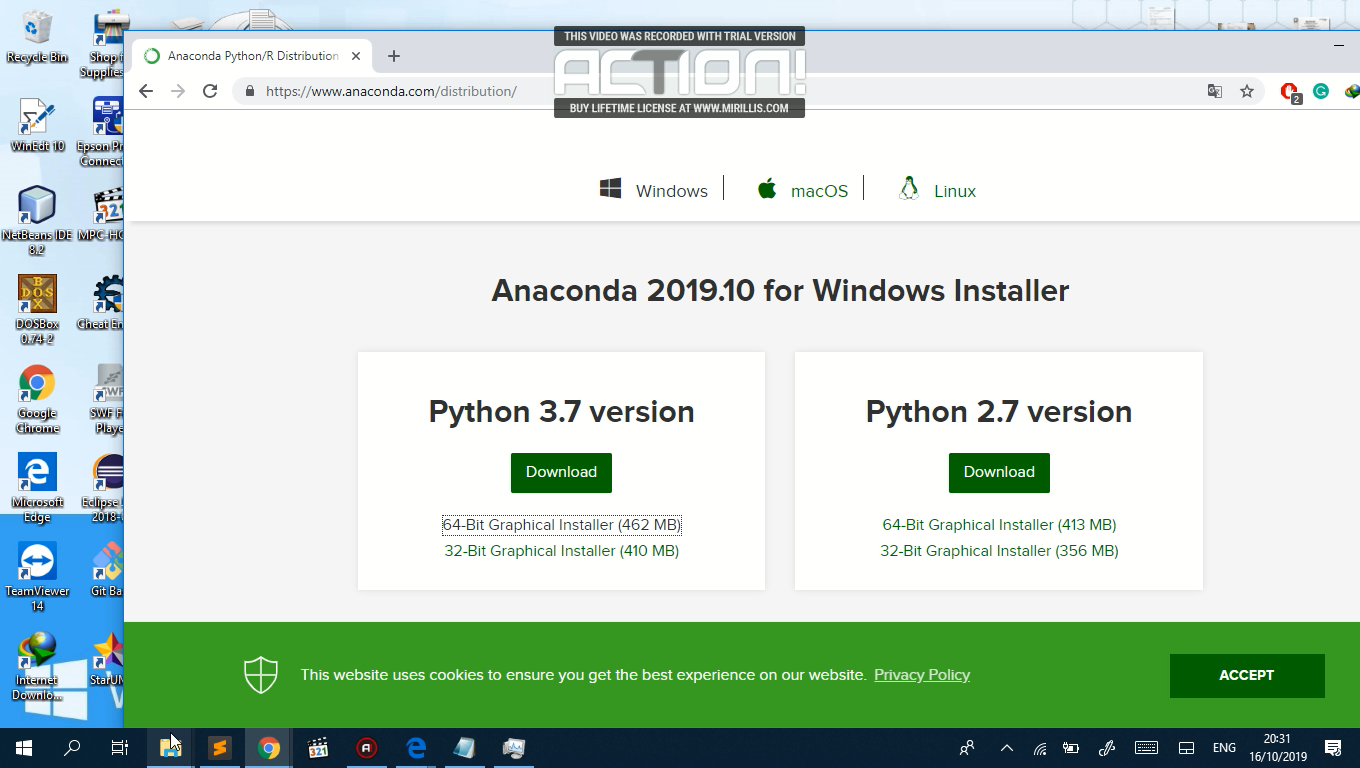
\includegraphics[width=8cm]{figures/1.png}	
\end{figure}

\begin{figure}[H]
	\centering
	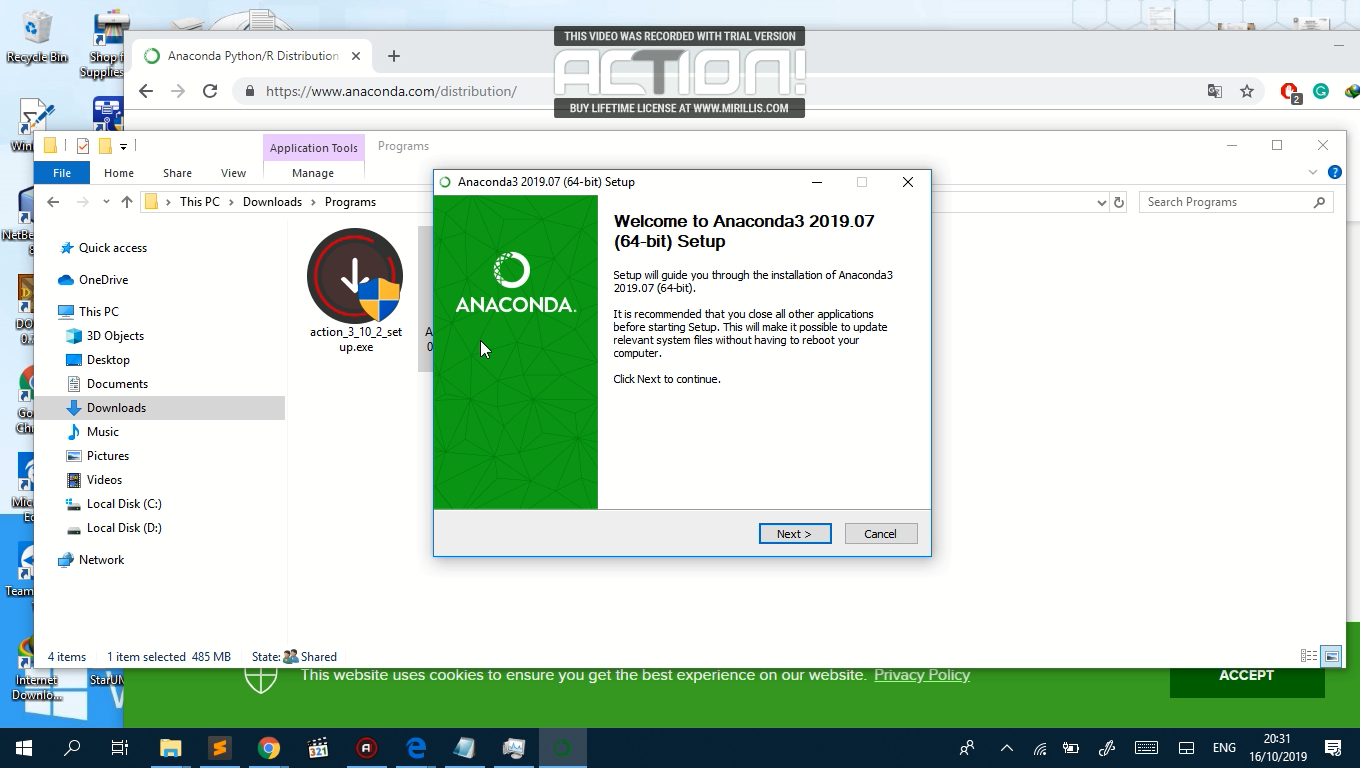
\includegraphics[width=8cm]{figures/2.png}
\end{figure}

\begin{figure}[H]
	\centering
	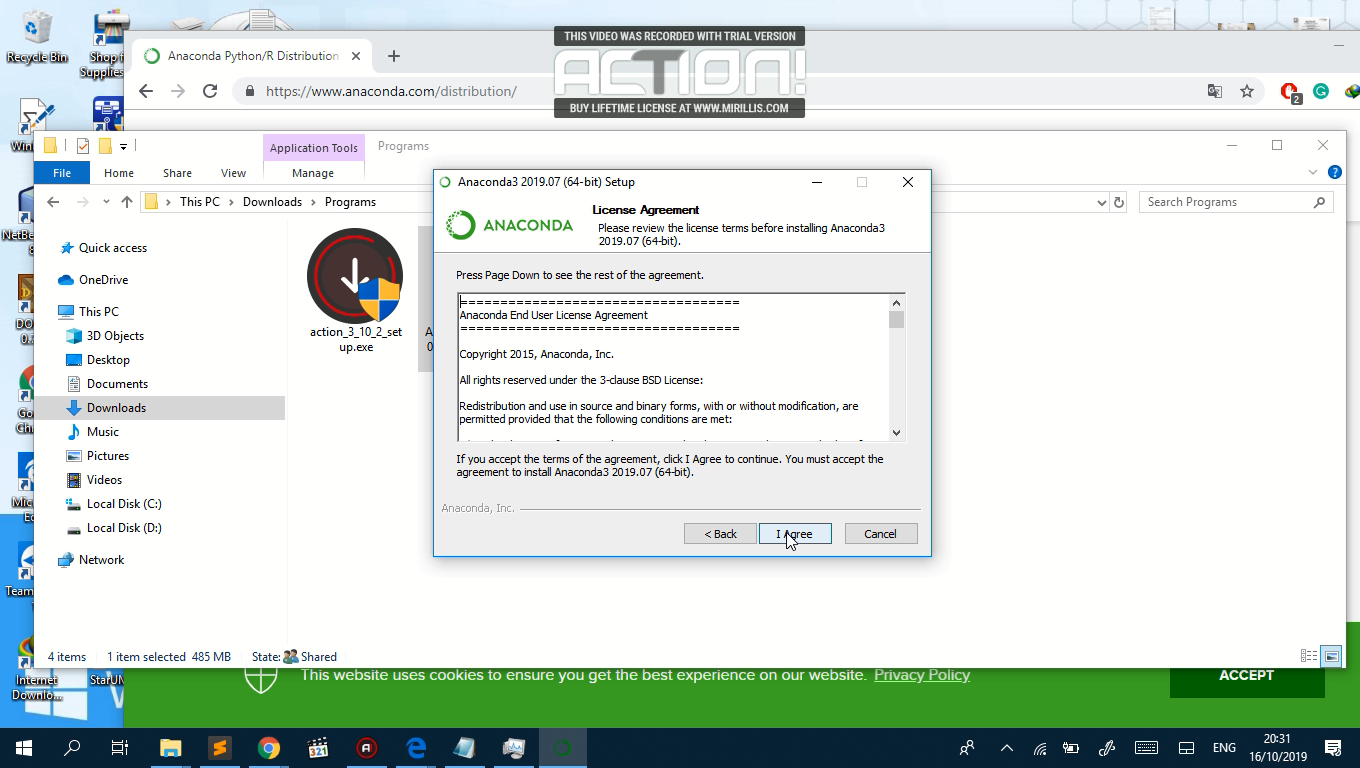
\includegraphics[width=8cm]{figures/3.png}
\end{figure}

\begin{figure}[H]
	\centering
	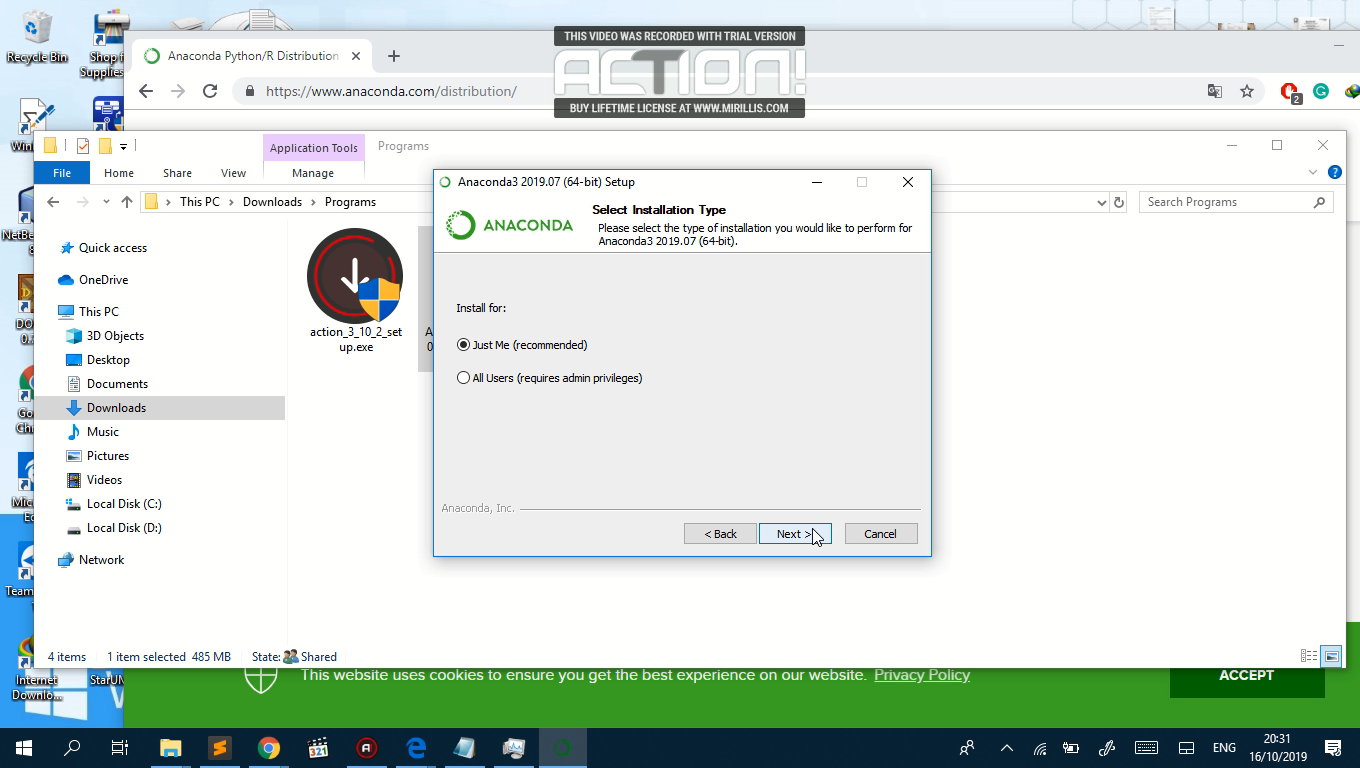
\includegraphics[width=8cm]{figures/4.png}
\end{figure}

\begin{figure}[H]
	\centering
	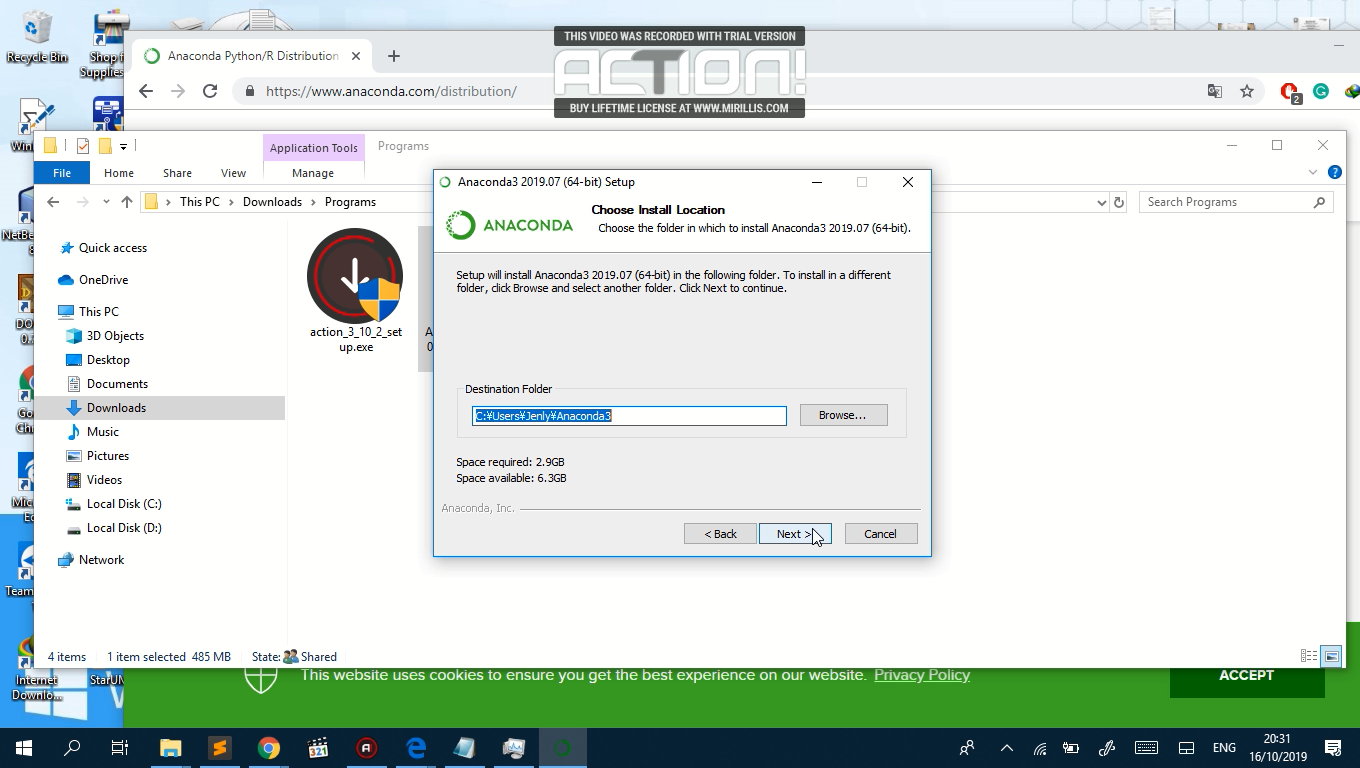
\includegraphics[width=8cm]{figures/5.png}
\end{figure}

\begin{figure}[H]
	\centering
	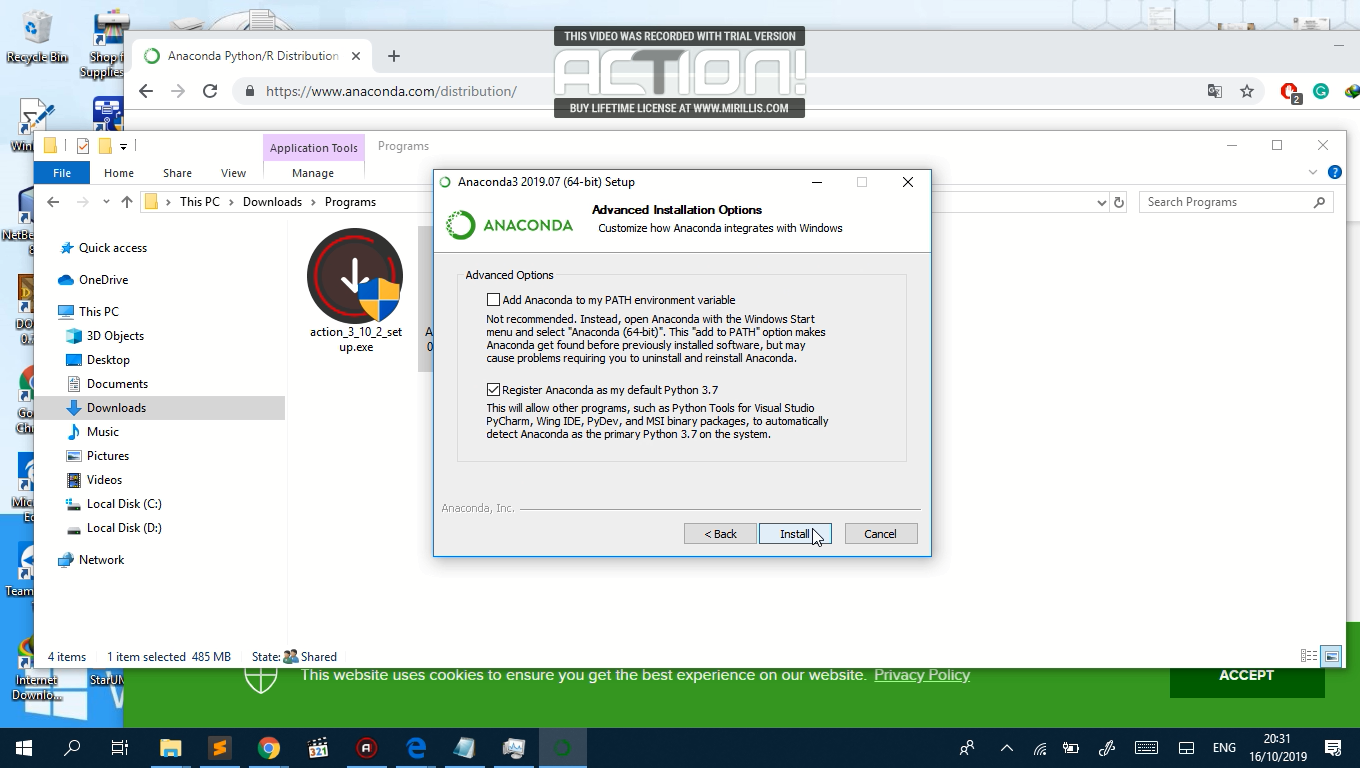
\includegraphics[width=8cm]{figures/6.png}
\end{figure}

\begin{figure}[H]
	\centering
	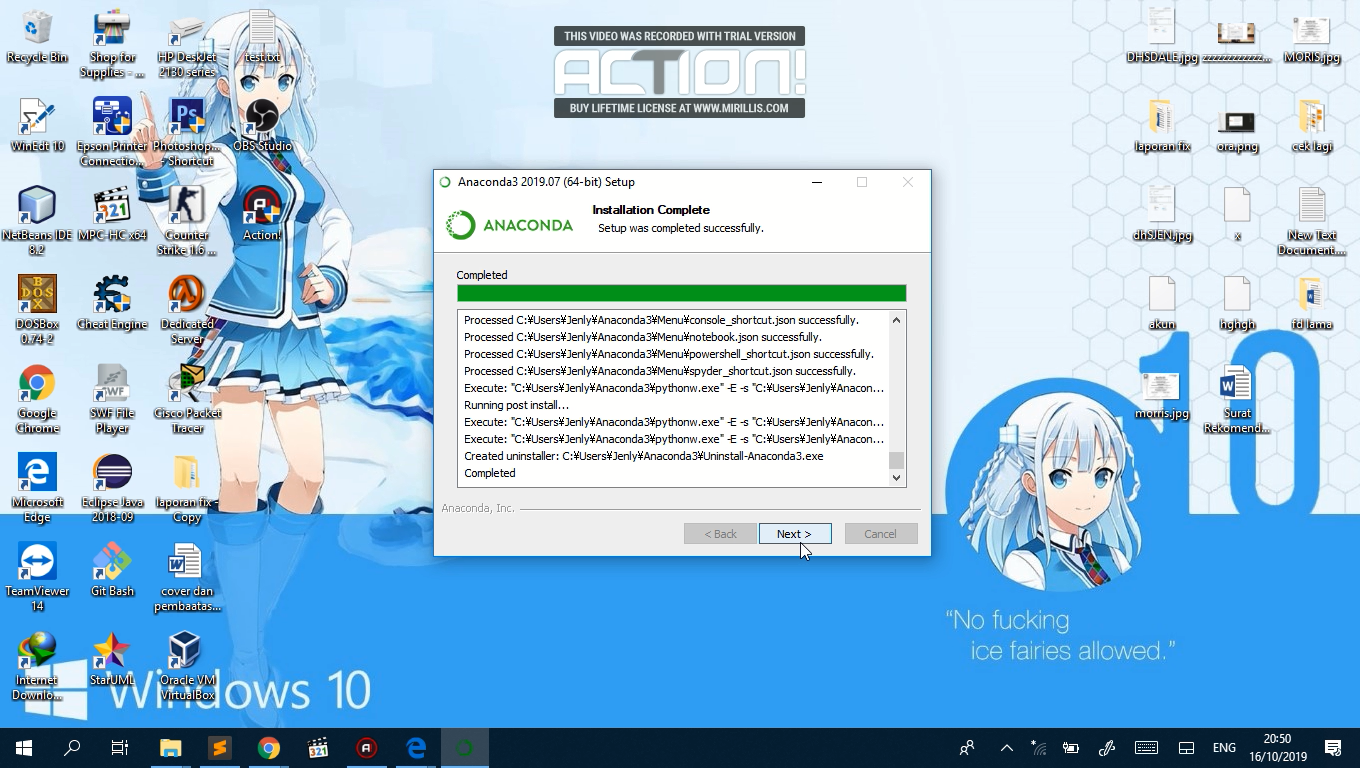
\includegraphics[width=8cm]{figures/7.png}
\end{figure}

\section{Instalasi python 3}
pertama download terlebih dahulu aplikasi nya kemudian klik untuk install.

\section{Cara Setting Enviroment}
pertama salin lokasi folder instalasi  anaconda . kemudian buka system di control panel. setelah itu klik advance sistem setting. kemudian klik enviroment variable. kemudian tambahkan link folder tadi di path. untuk langkah bisa lihat dibawah.
\begin{figure}[H]
	\centering
	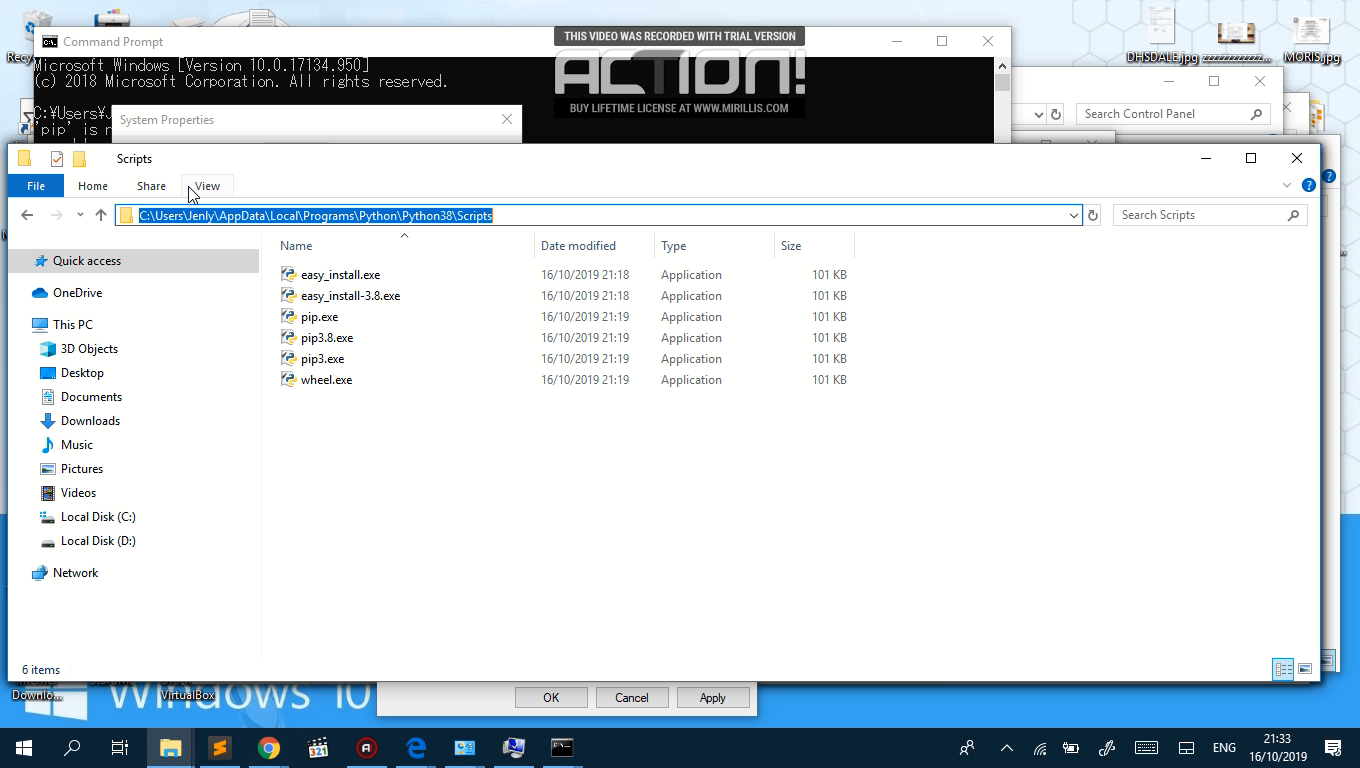
\includegraphics[width=8cm]{figures/3-1.png}
		
\end{figure}
\begin{figure}[H]
	\centering
	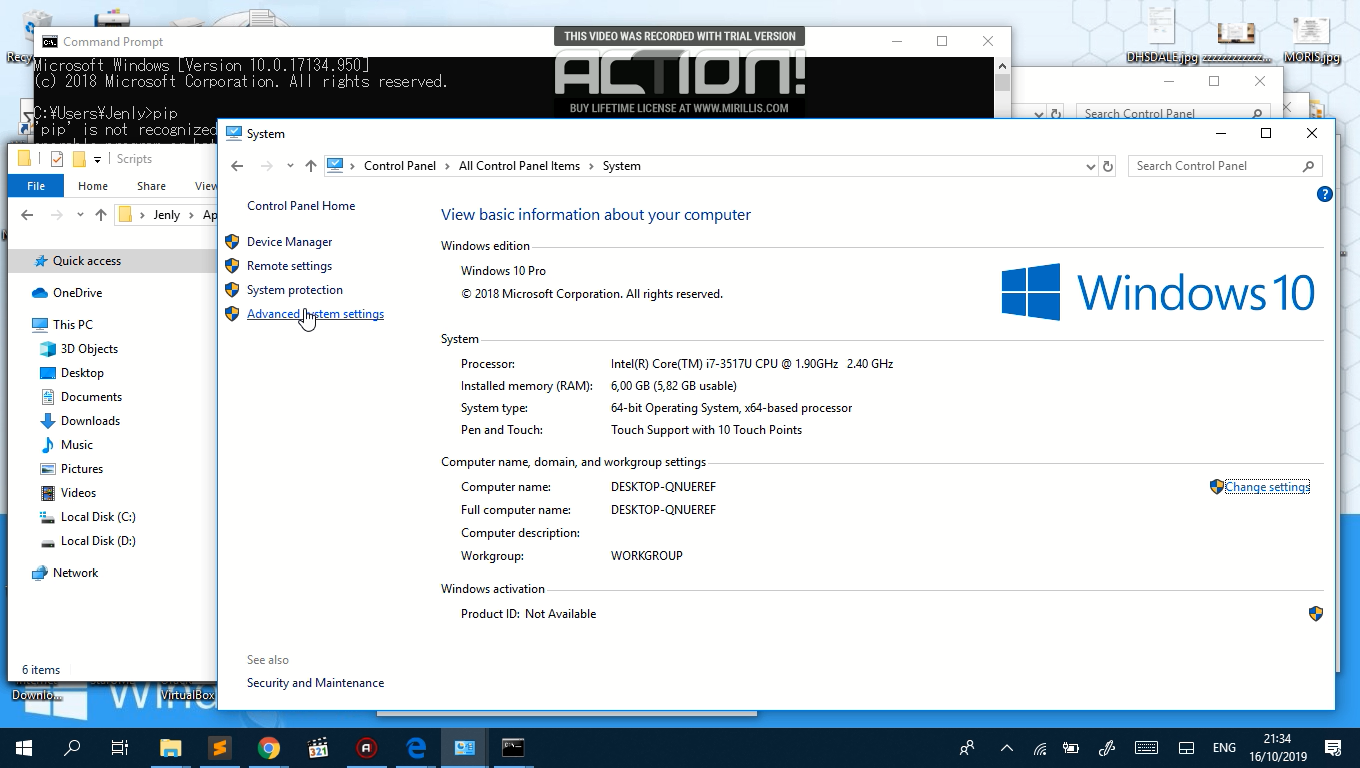
\includegraphics[width=8cm]{figures/3-2.png}
	
\end{figure}
\begin{figure}[H]
	\centering
	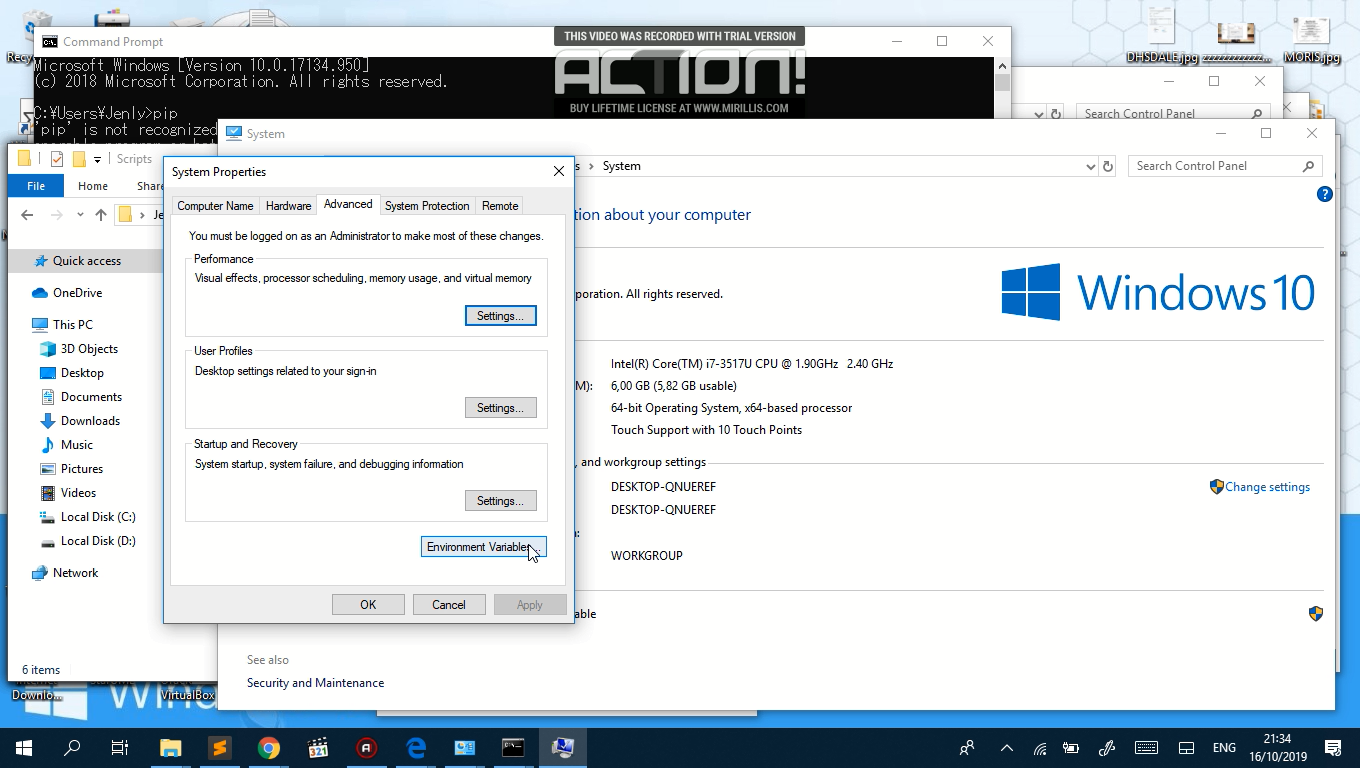
\includegraphics[width=8cm]{figures/3-3.png}
	
\end{figure}
\begin{figure}[H]
	\centering
	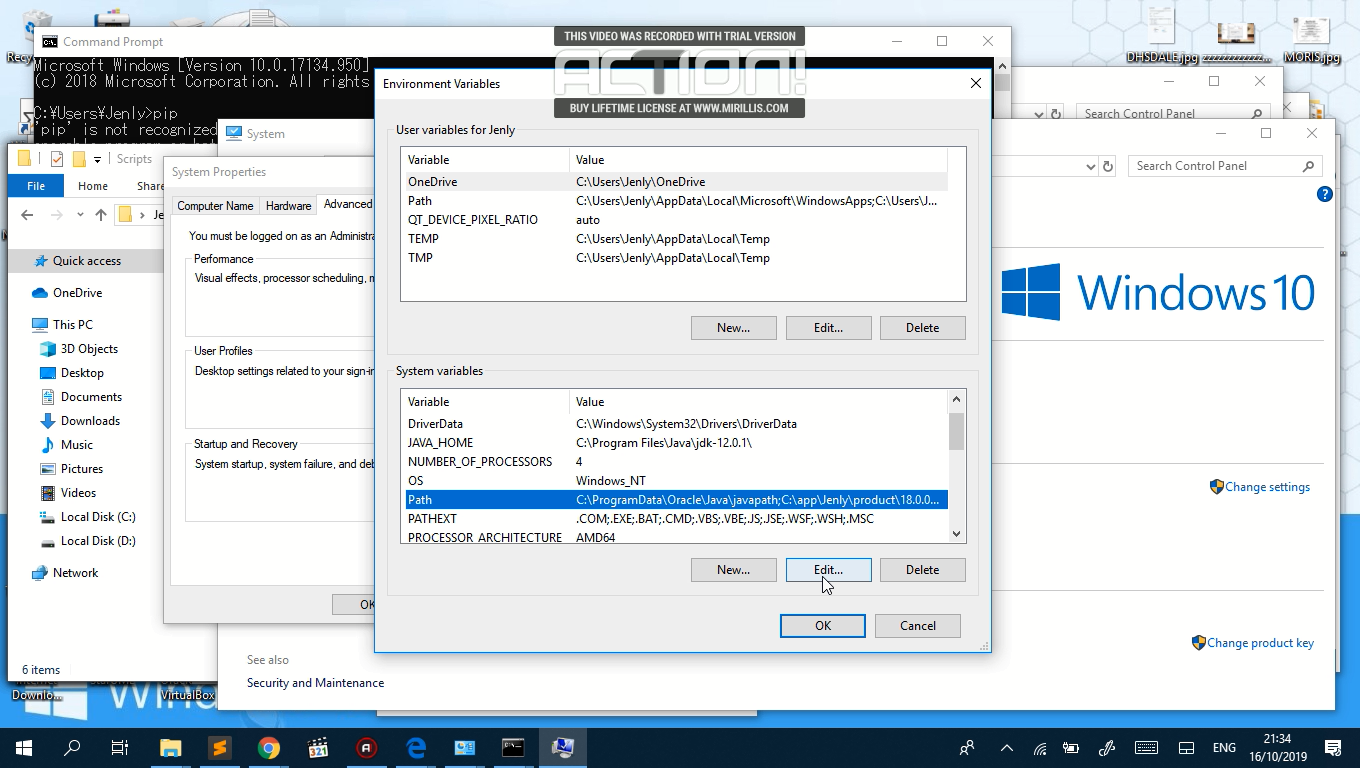
\includegraphics[width=8cm]{figures/3-4.png}
	\end{figure}
	
\begin{figure}[H]
	\centering
	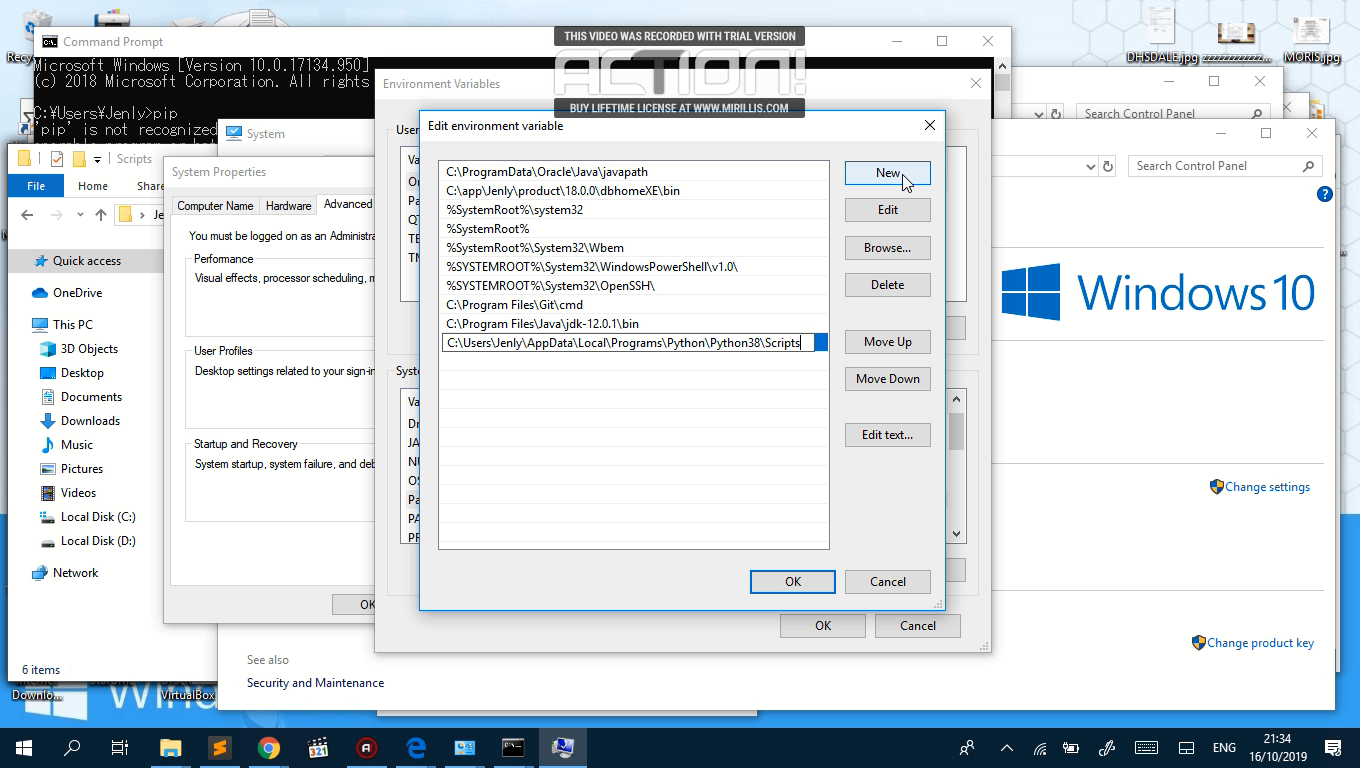
\includegraphics[width=8cm]{figures/3-5.png}
	
\end{figure}

\section{Entrepreter/cli melakui terminal atau cmd windows}
pertama buka command prompt. setelah itu ketik pip. kemudian tekan enter. untuk gambar nya bisa lihat dibawah.
\begin{figure}[H]
	\centering
	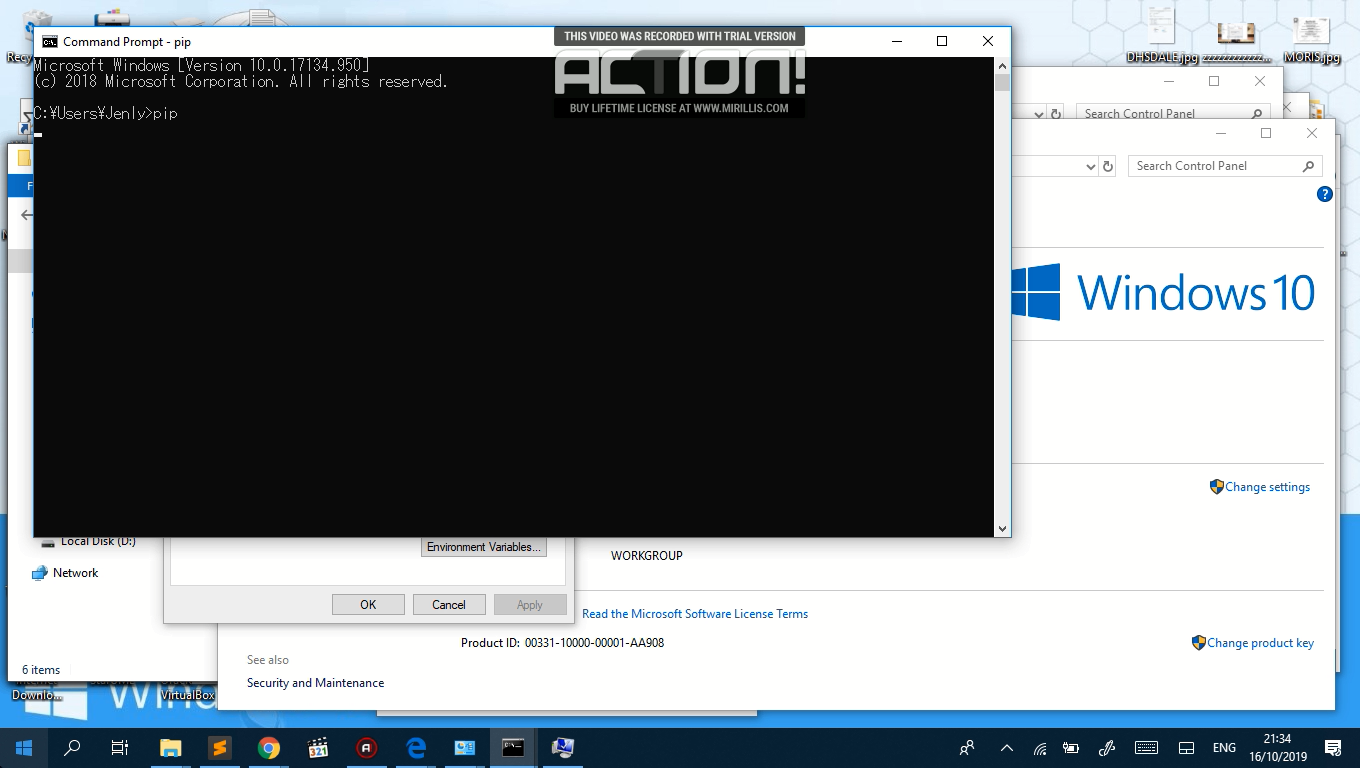
\includegraphics[width=8cm]{figures/4-1.png}
\end{figure}

\begin{figure}[H]
	\centering
	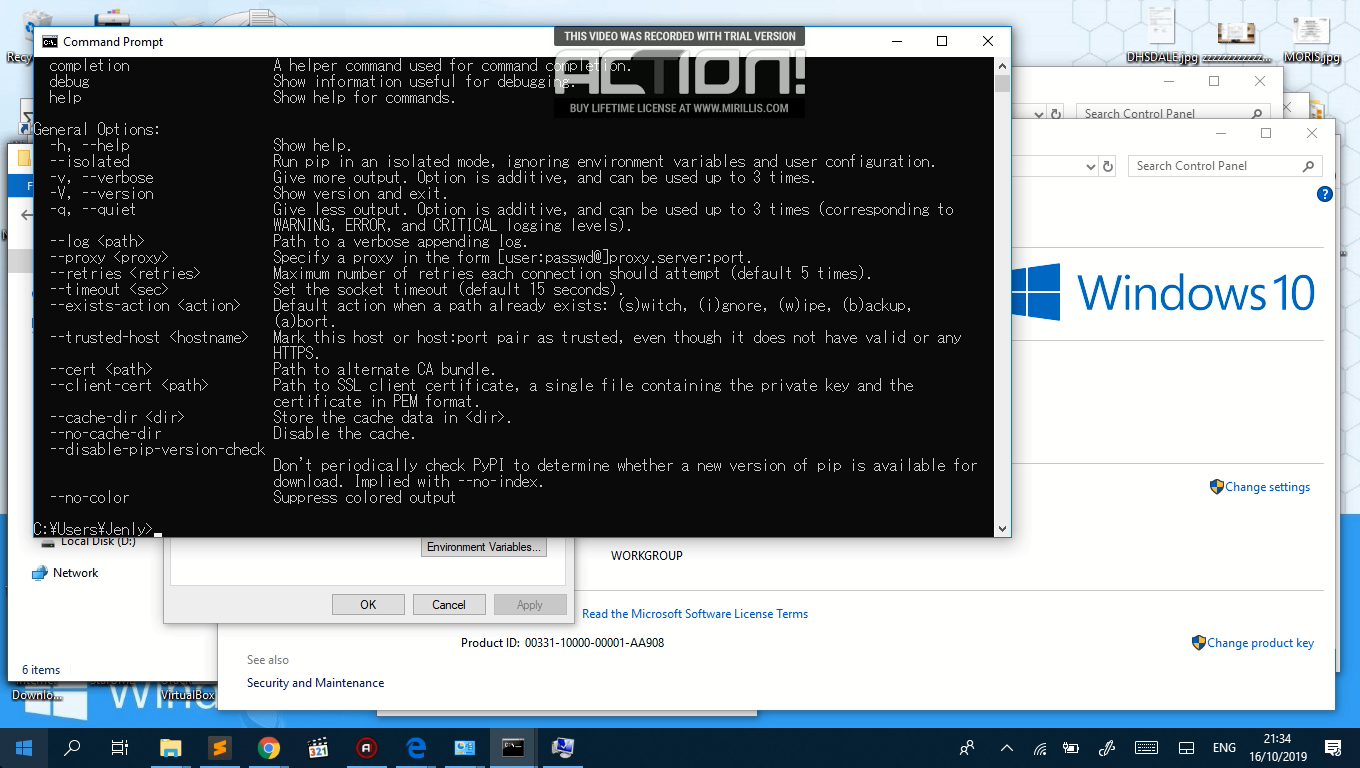
\includegraphics[width=8cm]{figures/4-2.png}
\end{figure}

\section{menjalankan dan mengupdate anaconda dan spyder}
	buka anaconda prompt. lalu klik conda update conda, tunggu sampai selesai kemudian klik enter ketika muncul procces(y/n). hal tersebut berlaku juga untuk update spyder. digambar di proses spyder tdk saya klik y karena spyder saya sudah versi terbaru. dan jika seandainya di klik ya maka terjadi adalah downgraded menyeluruh. berikut langkahnya.
\begin{figure}[H]
	\centering
	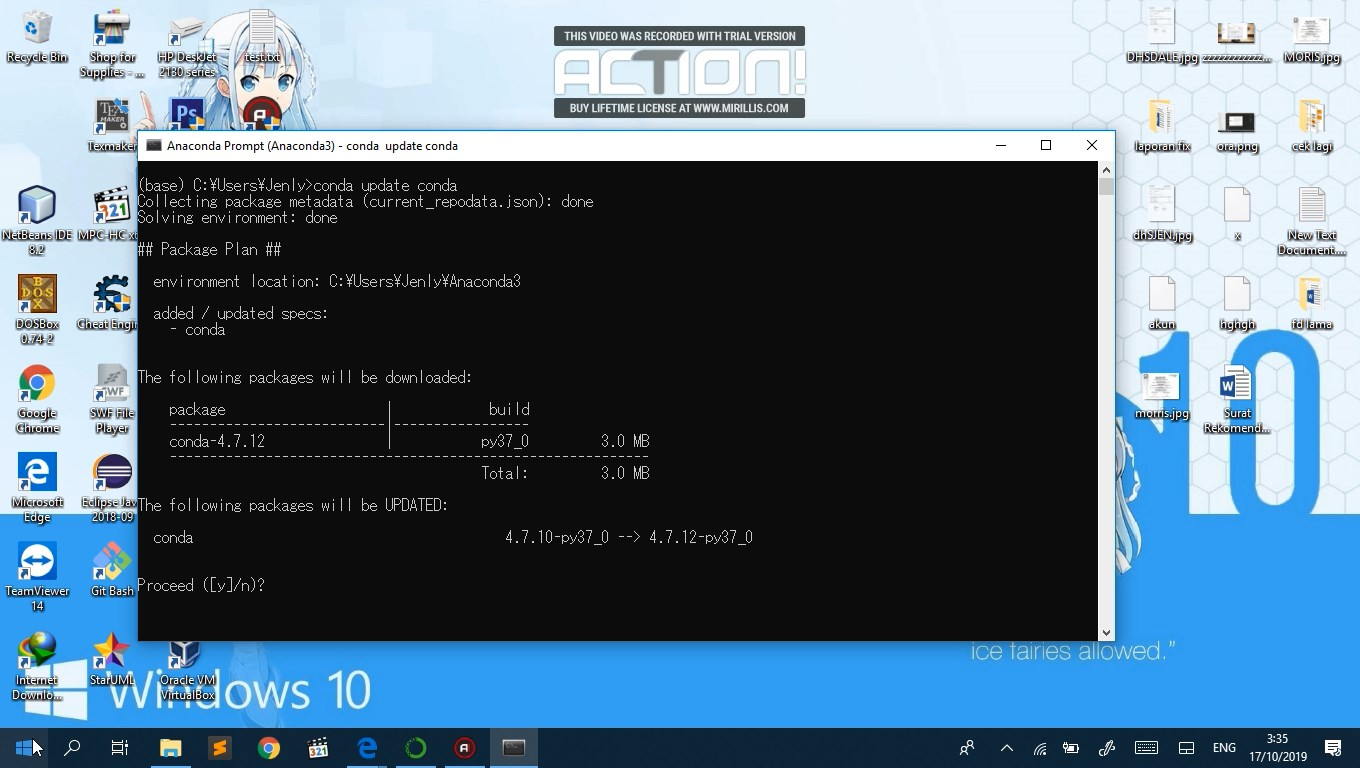
\includegraphics[width=8cm]{figures/6-6.jpg}
\end{figure}

\begin{figure}[H]
	\centering
	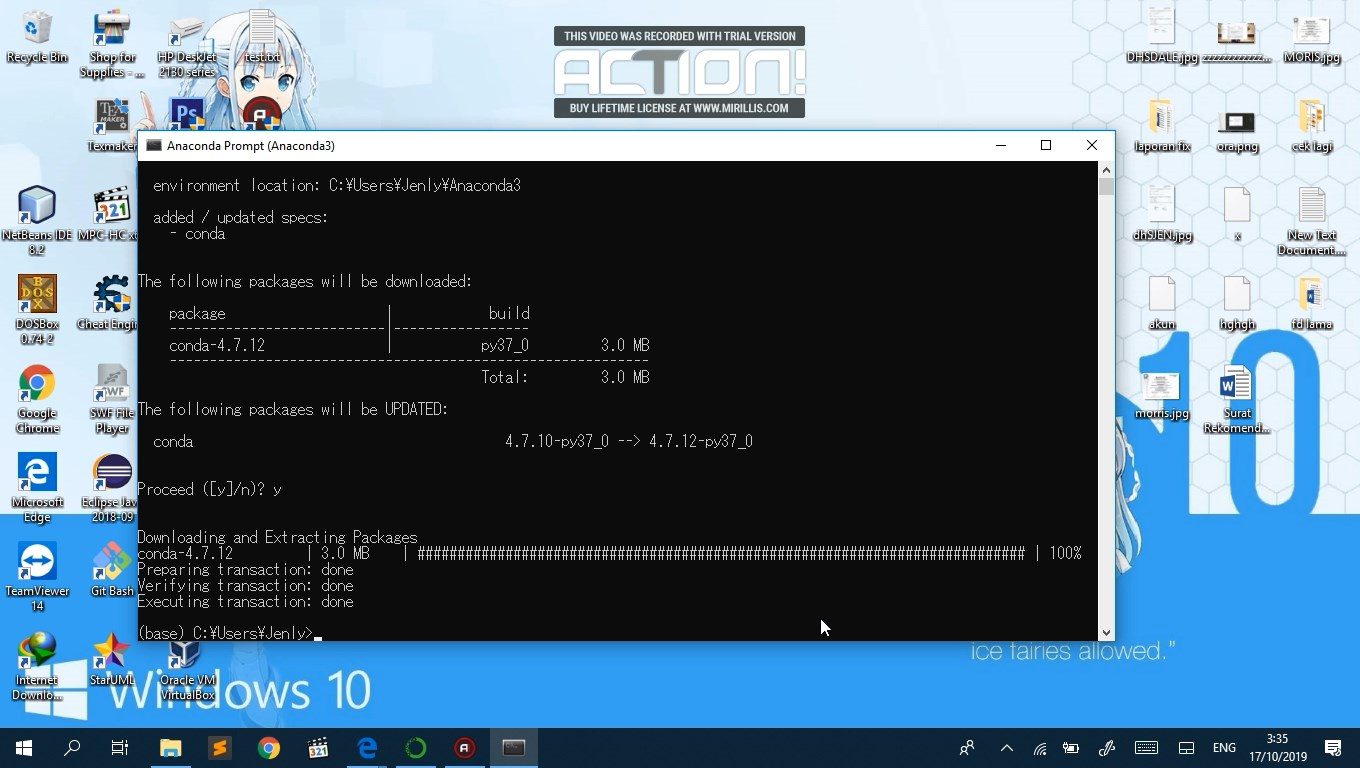
\includegraphics[width=8cm]{figures/6-7.jpg}
\end{figure}

\begin{figure}[H]
	\centering
	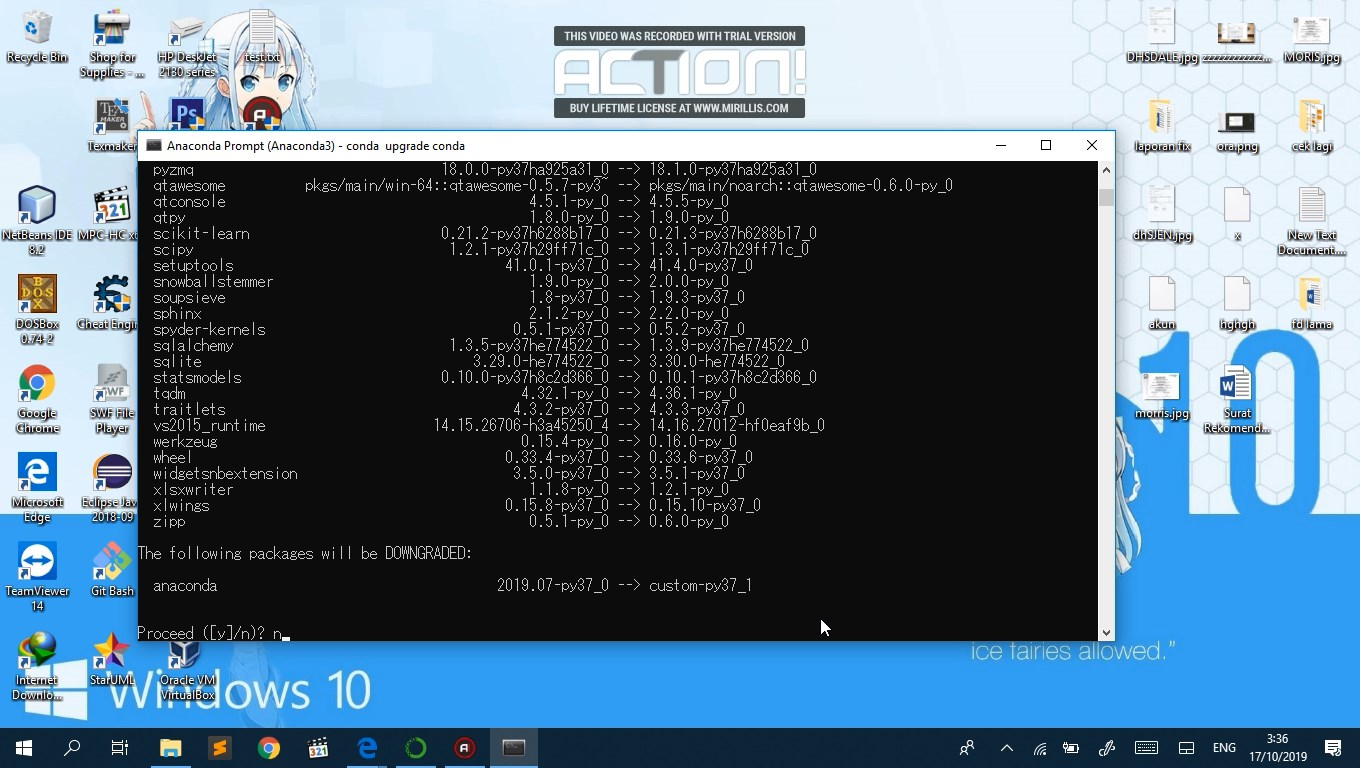
\includegraphics[width=8cm]{figures/6-8.jpg}
\end{figure}

\begin{figure}[H]
	\centering
	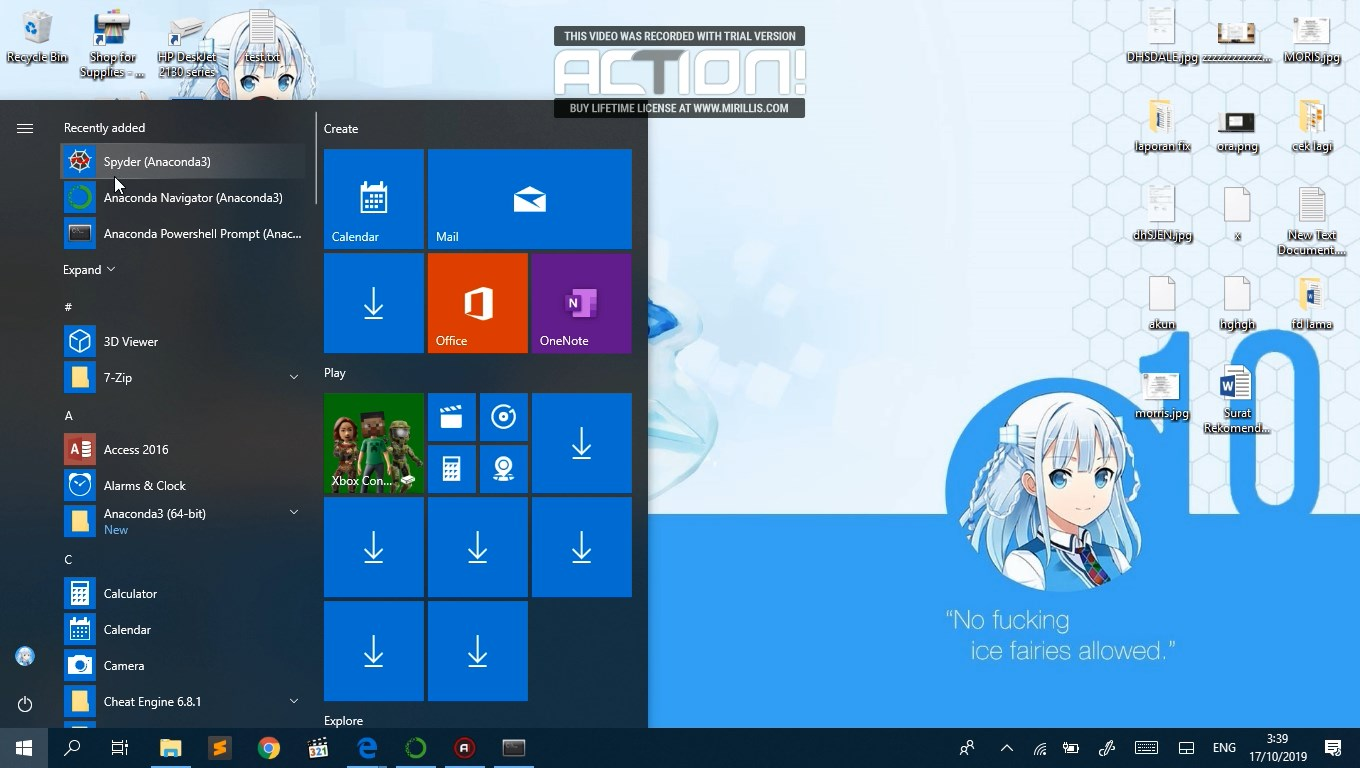
\includegraphics[width=8cm]{figures/6-9.jpg}
\end{figure}

\begin{figure}[H]
	\centering
	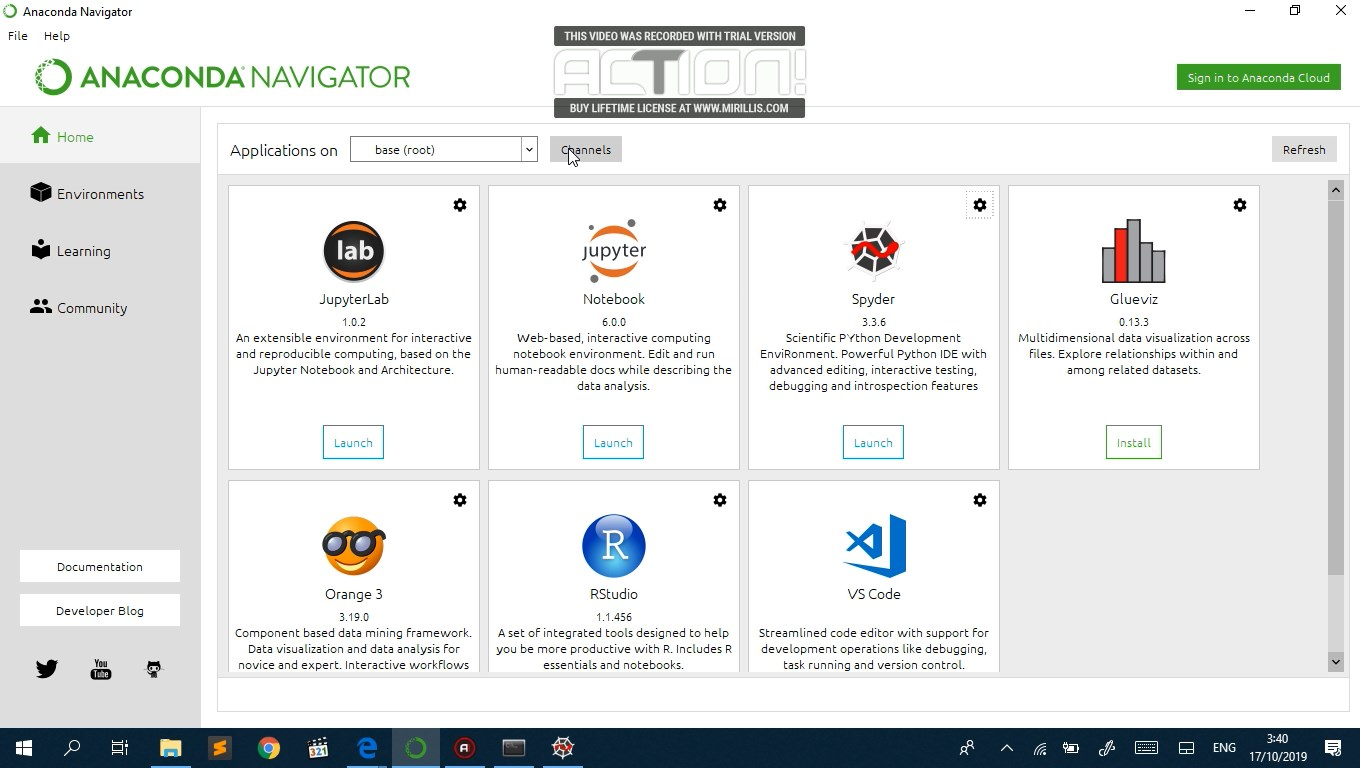
\includegraphics[width=8cm]{figures/6-10.jpg}
\end{figure}

\section{cara menjalankan script hello world di spyder}
	salin skrip dibawah ini. skrip dibawah bisa digunakan untuk python ver 2 dan 3
\begin{figure}[H]
	\centering
	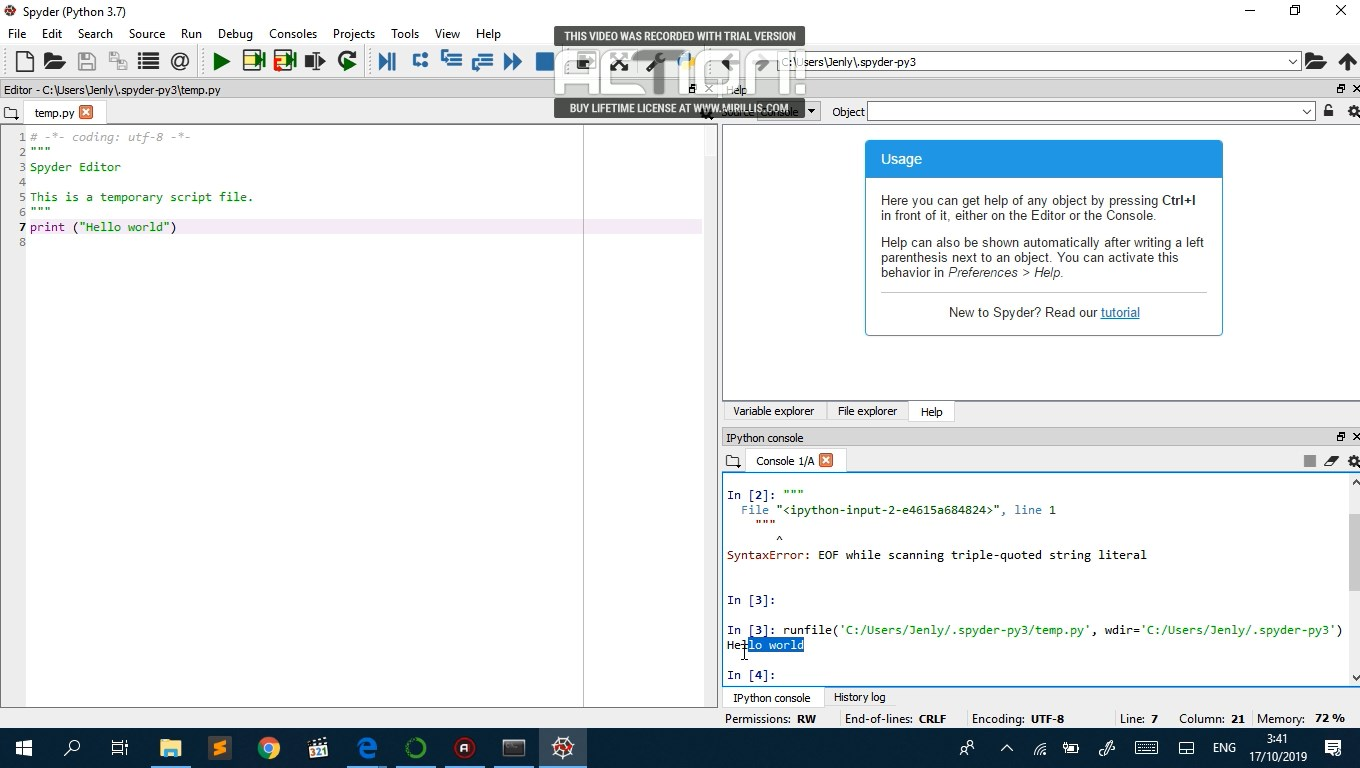
\includegraphics[width=8cm]{figures/he.jpg}
\end{figure}

\section{Cara menjalankan script login otomatis menggunakan selenium}
	pertama tulis script import untuk selenium. setelah itu buat skrip dibawah ini. gunakan inspect elemen untuk melihat struktur nya. lalu get ke web portal siap.
\begin{figure}[H]
	\centering
	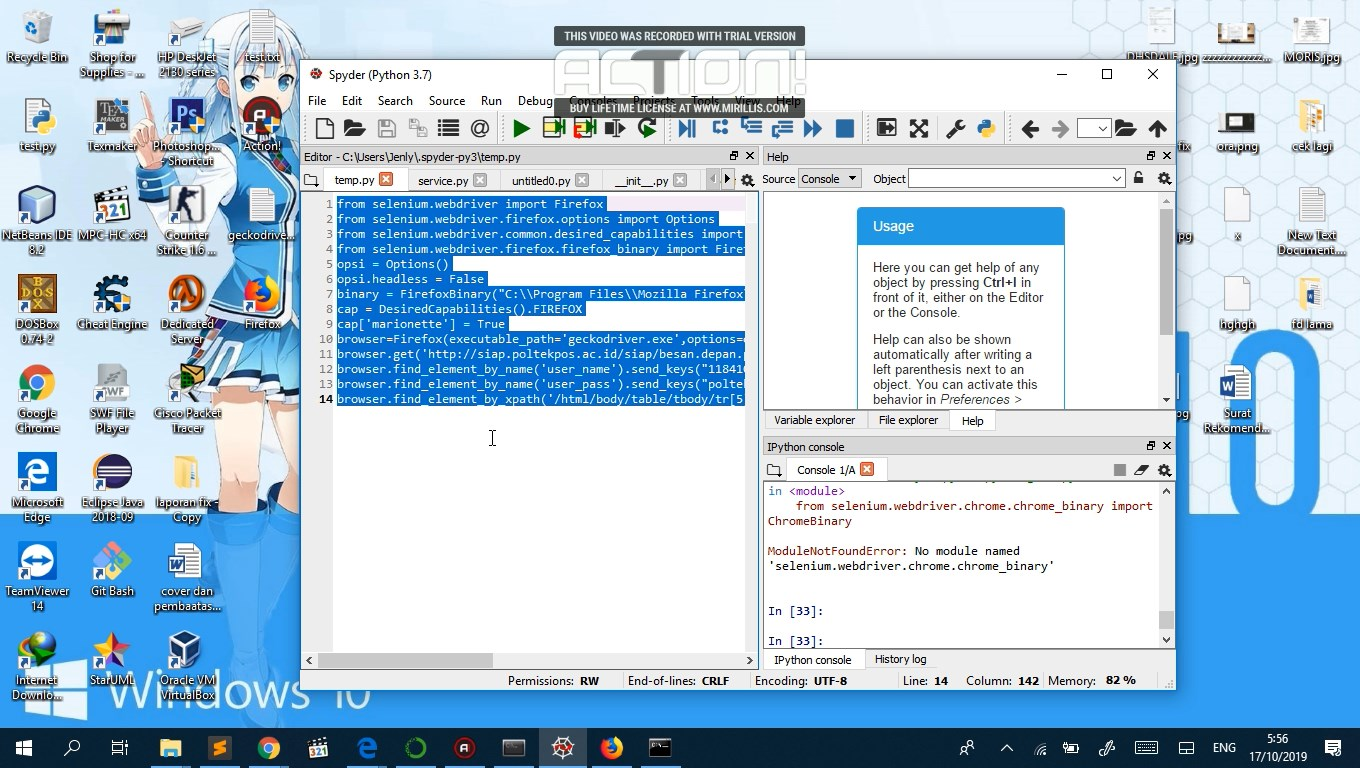
\includegraphics[width=8cm]{figures/rush.jpg}
\end{figure}

\section{cara memakai variable explorer di spyder}
pertama buat source seperti berikut ini. ketika di running klik variable explorer. di variable explorer kita bisa mengetahui tipe data yang digunakan. sehingga kita tidak kesulitan menentuka type datanya.
\begin{figure}[H]
	\centering
	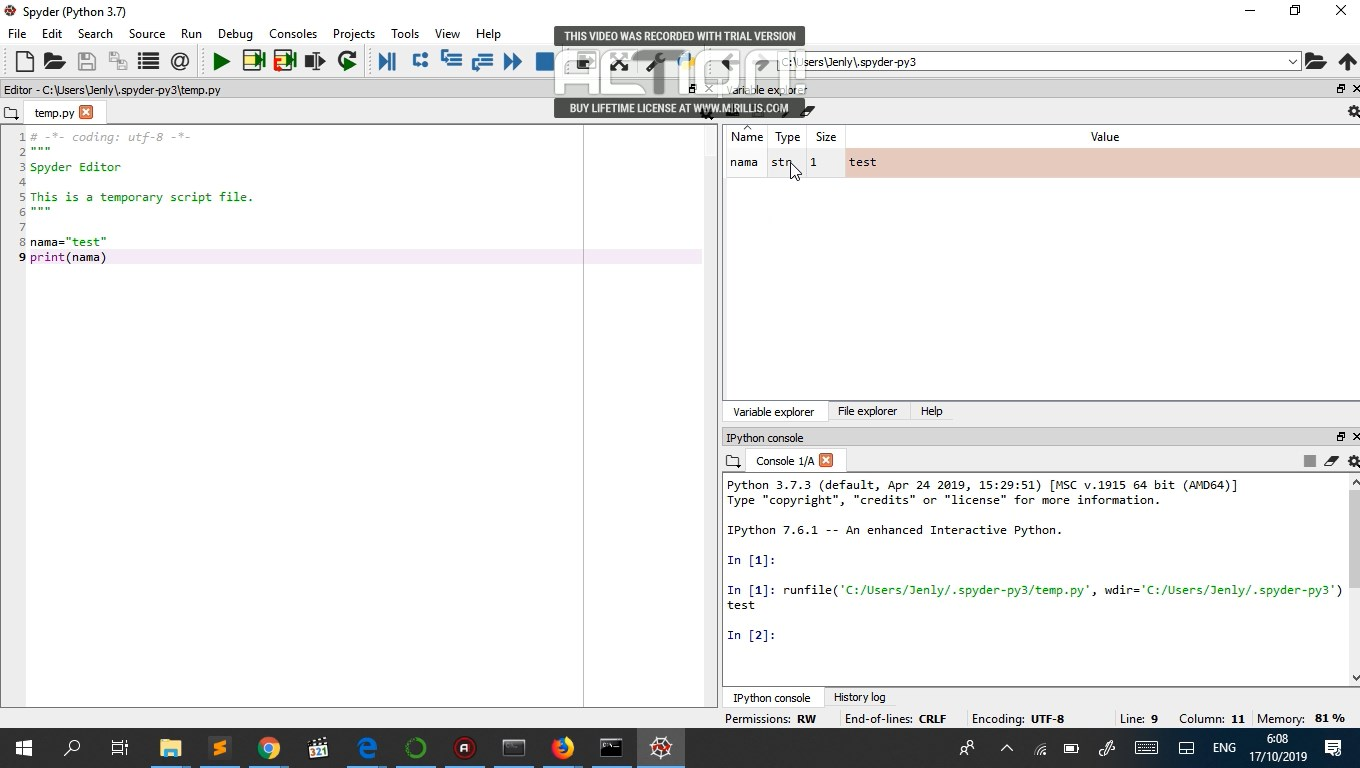
\includegraphics[width=8cm]{figures/far.jpg}
\end{figure}
